\section{Additional Results}
\label{app:additional_results}

This appendix extends the results of \S\ref{sec:findings}--\S\ref{sec:deployment}. Unless stated otherwise, results use Qwen3-VL-8B at \textbf{TLV} with gold pages on MMLongBench-Doc.

% The floats of B.1 to B.3 are declared here, ahead of their text and in the order of the
% subsections (representation, selection, reasoning), so they sit at the tops of text pages.
% GENERATED by ops/scripts/tables/ -- do not edit by hand, re-run the script.
% Numbers read from results/tables/mmlongbench/parser_scan_source.csv.
\definecolor{accteal}{HTML}{1BAF7A}
\begin{table}[t]
\centering
\small
\adjustbox{max width=\columnwidth}{%
\setlength{\tabcolsep}{6pt}%
\begin{tabular}{@{}l rr rr@{}}
\toprule
 & \multicolumn{2}{c}{\textbf{Born-digital}} & \multicolumn{2}{c}{\textbf{Scanned}} \\
\cmidrule(lr){2-3}\cmidrule(l){4-5}
\textbf{Text source} & \textbf{Text} & \textbf{+Image} & \textbf{Text} & \textbf{+Image} \\
\midrule
\multicolumn{5}{@{}l}{\emph{PaddleOCR-VL}} \\
\quad Text & \cellcolor{accteal!42}50.9 & \cellcolor{accteal!46}54.9 & \cellcolor{accteal!30}35.4 & \cellcolor{accteal!46}55.4 \\
\quad Layout & \cellcolor{accteal!37}43.8 & \cellcolor{accteal!40}47.5 & \cellcolor{accteal!22}26.3 & \cellcolor{accteal!48}57.9 \\
\quad Table & \cellcolor{accteal!40}47.6 & \cellcolor{accteal!39}46.5 & \cellcolor{accteal!50}59.4 & \cellcolor{accteal!60}71.9 \\
\quad Chart & \cellcolor{accteal!20}23.8 & \cellcolor{accteal!34}40.8 & \cellcolor{accteal!4}4.2 & \cellcolor{accteal!45}54.2 \\
\quad Figure & \cellcolor{accteal!15}17.4 & \cellcolor{accteal!31}37.0 & \cellcolor{accteal!26}31.1 & \cellcolor{accteal!48}57.5 \\
\quad \textbf{All} & \cellcolor{accteal!33}40.1 & \cellcolor{accteal!41}49.7 & \cellcolor{accteal!27}32.8 & \cellcolor{accteal!51}61.2 \\
\midrule
\multicolumn{5}{@{}l}{\emph{MinerU 2.5}} \\
\quad Text & \cellcolor{accteal!25}30.1 & \cellcolor{accteal!41}49.1 & \cellcolor{accteal!26}30.8 & \cellcolor{accteal!45}53.8 \\
\quad Layout & \cellcolor{accteal!17}20.0 & \cellcolor{accteal!37}43.8 & \cellcolor{accteal!15}18.4 & \cellcolor{accteal!42}50.0 \\
\quad Table & \cellcolor{accteal!31}36.8 & \cellcolor{accteal!36}42.7 & \cellcolor{accteal!47}56.2 & \cellcolor{accteal!55}65.6 \\
\quad Chart & \cellcolor{accteal!15}17.7 & \cellcolor{accteal!32}38.5 & \cellcolor{accteal!12}14.6 & \cellcolor{accteal!40}47.9 \\
\quad Figure & \cellcolor{accteal!10}12.5 & \cellcolor{accteal!32}38.6 & \cellcolor{accteal!21}25.5 & \cellcolor{accteal!42}50.9 \\
\quad \textbf{All} & \cellcolor{accteal!22}26.6 & \cellcolor{accteal!38}46.0 & \cellcolor{accteal!23}27.4 & \cellcolor{accteal!46}55.7 \\
\midrule
\multicolumn{5}{@{}l}{\emph{Unlimited-OCR}} \\
\quad Text & \cellcolor{accteal!42}50.4 & \cellcolor{accteal!44}53.1 & \cellcolor{accteal!31}36.9 & \cellcolor{accteal!47}56.9 \\
\quad Layout & \cellcolor{accteal!37}43.8 & \cellcolor{accteal!44}52.5 & \cellcolor{accteal!31}36.8 & \cellcolor{accteal!50}60.5 \\
\quad Table & \cellcolor{accteal!41}49.7 & \cellcolor{accteal!40}48.1 & \cellcolor{accteal!50}59.4 & \cellcolor{accteal!60}71.9 \\
\quad Chart & \cellcolor{accteal!20}23.8 & \cellcolor{accteal!35}42.3 & \cellcolor{accteal!2}2.1 & \cellcolor{accteal!49}58.3 \\
\quad Figure & \cellcolor{accteal!17}20.7 & \cellcolor{accteal!32}38.0 & \cellcolor{accteal!28}34.0 & \cellcolor{accteal!49}58.5 \\
\quad \textbf{All} & \cellcolor{accteal!35}42.3 & \cellcolor{accteal!42}50.2 & \cellcolor{accteal!29}34.3 & \cellcolor{accteal!53}63.7 \\
\midrule
\multicolumn{5}{@{}l}{\emph{PyMuPDF}} \\
\quad Text & \cellcolor{accteal!42}50.0 & \cellcolor{accteal!45}54.4 & \cellcolor{accteal!3}3.1 & \cellcolor{accteal!42}50.8 \\
\quad Layout & \cellcolor{accteal!33}40.0 & \cellcolor{accteal!40}47.5 & \cellcolor{accteal!2}2.6 & \cellcolor{accteal!44}52.6 \\
\quad Table & \cellcolor{accteal!40}48.1 & \cellcolor{accteal!37}44.9 & \cellcolor{accteal!0}0.0 & \cellcolor{accteal!50}59.4 \\
\quad Chart & \cellcolor{accteal!21}24.6 & \cellcolor{accteal!31}37.7 & \cellcolor{accteal!0}0.0 & \cellcolor{accteal!45}54.2 \\
\quad Figure & \cellcolor{accteal!16}19.6 & \cellcolor{accteal!34}41.3 & \cellcolor{accteal!6}7.5 & \cellcolor{accteal!44}52.8 \\
\quad \textbf{All} & \cellcolor{accteal!34}40.6 & \cellcolor{accteal!41}49.7 & \cellcolor{accteal!3}4.0 & \cellcolor{accteal!48}57.7 \\
\bottomrule
\end{tabular}%
}
\caption{Accuracy by text source, evidence source and scan status. Accuracy (\%) on answerable MMLongBench-Doc questions with gold pages, with the text alone and with the page image added.}
\label{tab:app_parser_sources}
\end{table}
% {\footnotesize\raggedright
% Qwen3-VL-8B bf16, medium resolution, no instruction, accuracy judge. The \textbf{All} rows
% are the bars of the fidelity figure. Source rows overlap, so \textbf{All} pools each
% question once. Scan status is the hand label (646 born-digital, 201 scanned questions).\par}

% GENERATED by ops/scripts/tables/ -- do not edit by hand, re-run the script.
% Numbers read from results/tables/mmlongbench/resolution_source.csv.
\definecolor{accteal}{HTML}{1BAF7A}
\begin{table}[t]
\centering
\small
\adjustbox{max width=\columnwidth}{%
\setlength{\tabcolsep}{5pt}%
\begin{tabular}{@{}l rrr @{\hskip 10pt} rrr@{}}
\toprule
 & \multicolumn{3}{c}{\textbf{TLV}} & \multicolumn{3}{c}{\textbf{V}} \\
\cmidrule(lr){2-4}\cmidrule(l){5-7}
\textbf{Source} & \texttt{low} & \texttt{med} & \texttt{high} & \texttt{low} & \texttt{med} & \texttt{high} \\
\midrule
Text & \cellcolor{accteal!56}52.9 & \cellcolor{accteal!60}55.0 & \cellcolor{accteal!60}55.0 & \cellcolor{accteal!27}38.8 & \cellcolor{accteal!41}45.4 & \cellcolor{accteal!53}51.5 \\
Layout & \cellcolor{accteal!43}46.6 & \cellcolor{accteal!50}50.0 & \cellcolor{accteal!58}54.2 & \cellcolor{accteal!45}47.5 & \cellcolor{accteal!48}49.2 & \cellcolor{accteal!57}53.4 \\
Table & \cellcolor{accteal!47}48.8 & \cellcolor{accteal!49}49.8 & \cellcolor{accteal!47}48.8 & \cellcolor{accteal!0}25.3 & \cellcolor{accteal!24}37.3 & \cellcolor{accteal!35}42.4 \\
Chart & \cellcolor{accteal!26}38.2 & \cellcolor{accteal!40}44.9 & \cellcolor{accteal!46}48.3 & \cellcolor{accteal!18}34.3 & \cellcolor{accteal!40}44.9 & \cellcolor{accteal!46}48.3 \\
Figure & \cellcolor{accteal!29}39.7 & \cellcolor{accteal!41}45.5 & \cellcolor{accteal!46}48.3 & \cellcolor{accteal!26}38.3 & \cellcolor{accteal!30}40.0 & \cellcolor{accteal!37}43.8 \\
\midrule
\textbf{All} & \cellcolor{accteal!48}49.2 & \cellcolor{accteal!55}52.5 & \cellcolor{accteal!59}54.7 & \cellcolor{accteal!25}37.8 & \cellcolor{accteal!41}45.7 & \cellcolor{accteal!50}50.2 \\
\bottomrule
\end{tabular}%
}
\caption{Accuracy by image resolution and evidence source. Accuracy (\%) on answerable MMLongBench-Doc questions with gold pages, with parser text (TLV) and without it (V).}
\label{tab:app_resolution_sources}
\end{table}
% {\footnotesize\raggedright
% Qwen3-VL-8B bf16, PaddleOCR-VL, no instruction, accuracy judge, all 847 answerable
% questions. Source rows overlap, so \textbf{All} pools each question once.\par}

% GENERATED by ops/scripts/tables/ -- do not edit by hand, re-run the script.
% Numbers read from results/tables/longdocurl/ldu_question_type.csv and ldu_headline.csv,
% results/tables/unified/unified_ladder.csv and docs/generated/longdocurl_stats.csv.
\definecolor{accteal}{HTML}{1BAF7A}
\begin{table}[t]
\centering
\small
\adjustbox{max width=\columnwidth}{%
\setlength{\tabcolsep}{5pt}%
\begin{tabular}{@{}l rrrr r@{}}
\toprule
\textbf{Task and question type} & \textbf{T} & \textbf{TL} & \textbf{TLV} & \textbf{V} & $n$ \\
\midrule
\emph{Understanding} (\texttt{extract}) & \cellcolor{accteal!51}74.1 & \cellcolor{accteal!54}77.1 & \cellcolor{accteal!59}\textbf{83.4} & \cellcolor{accteal!51}74.6 & 1{,}243 \\
\midrule
\emph{Locating} & \cellcolor{accteal!25}43.5 & \cellcolor{accteal!32}\textbf{51.6} & \cellcolor{accteal!30}50.0 & \cellcolor{accteal!26}45.4 & 695 \\
\quad \texttt{extract\_fig2tab} & \cellcolor{accteal!37}58.4 & \cellcolor{accteal!49}\textbf{71.6} & \cellcolor{accteal!41}62.3 & \cellcolor{accteal!35}55.4 & 231 \\
\quad \texttt{topic2title} & \cellcolor{accteal!11}27.9 & \cellcolor{accteal!12}28.8 & \cellcolor{accteal!17}\textbf{35.1} & \cellcolor{accteal!14}30.8 & 201 \\
\quad \texttt{summary2title} & \cellcolor{accteal!45}67.2 & \cellcolor{accteal!57}\textbf{81.1} & \cellcolor{accteal!54}77.2 & \cellcolor{accteal!51}74.3 & 137 \\
\quad \texttt{summary2tab} & \cellcolor{accteal!0}14.9 & \cellcolor{accteal!3}18.3 & \cellcolor{accteal!4}\textbf{19.6} & \cellcolor{accteal!4}19.0 & 126 \\
\midrule
\emph{Reasoning} & \cellcolor{accteal!45}66.8 & \cellcolor{accteal!45}67.5 & \cellcolor{accteal!50}\textbf{73.4} & \cellcolor{accteal!37}58.3 & 387 \\
\quad \texttt{calculate} & \cellcolor{accteal!40}61.0 & \cellcolor{accteal!45}66.7 & \cellcolor{accteal!50}\textbf{72.8} & \cellcolor{accteal!31}50.7 & 145 \\
\quad \texttt{count} & \cellcolor{accteal!37}57.9 & \cellcolor{accteal!36}56.2 & \cellcolor{accteal!44}\textbf{66.3} & \cellcolor{accteal!37}58.0 & 117 \\
\quad \texttt{compare} & \cellcolor{accteal!57}\textbf{81.1} & \cellcolor{accteal!55}78.8 & \cellcolor{accteal!56}80.2 & \cellcolor{accteal!43}65.2 & 112 \\
\quad \texttt{summarize} & \cellcolor{accteal!60}\textbf{84.6} & \cellcolor{accteal!53}76.9 & \cellcolor{accteal!58}81.8 & \cellcolor{accteal!60}\textbf{84.6} & 13 \\
\midrule
\textbf{All} & \cellcolor{accteal!42}63.7 & \cellcolor{accteal!46}68.0 & \cellcolor{accteal!49}\textbf{71.9} & \cellcolor{accteal!41}63.1 & 2{,}325 \\
\bottomrule
\end{tabular}%
}
\caption{LongDocURL accuracy by task and question type. Accuracy (\%) on answerable questions with gold pages; $n$ is the number of questions.}
\label{tab:app_ldu_types}
\end{table}
% {\footnotesize\raggedright
% Qwen3-VL-8B bf16, PaddleOCR-VL, medium resolution, no instruction, accuracy judge. The
% italic rows pool a task's question types. $n$ is the corpus count; a cell can sit on a
% few fewer questions.\par}


\begin{figure*}[t]
\centering
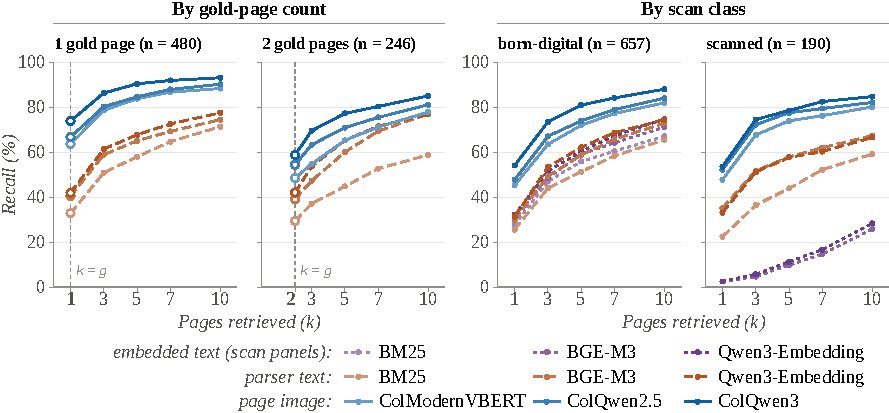
\includegraphics[width=0.95\textwidth]{appendix/figures/retrieval.pdf}
\caption{Page-level recall on MMLongBench-Doc by retrieval depth, split by gold-page count and by scan status.}
\label{fig:app_retrieval}
\end{figure*}

% GENERATED by ops/scripts/tables/ -- do not edit by hand, re-run the script.
% Numbers read from results/tables/longdocurl/ldu_selection_withholding.csv.
\definecolor{recwarm}{HTML}{D95926}
\definecolor{accteal}{HTML}{1BAF7A}
\begin{table}[t]
\centering
\small
\adjustbox{max width=\columnwidth}{%
\setlength{\tabcolsep}{3.5pt}%
\begin{tabular}{@{}l rr rr rr rr r@{}}
\toprule
 & \multicolumn{2}{c}{\textbf{Drop top}} & \multicolumn{2}{c}{\textbf{Drop bottom}} & \multicolumn{2}{c}{\textbf{Keep top}} & \multicolumn{2}{c}{\textbf{Keep bottom}} & \\
\cmidrule(lr){2-3}\cmidrule(lr){4-5}\cmidrule(lr){6-7}\cmidrule(lr){8-9}
\textbf{Source} & $-$ & $+$ & $-$ & $+$ & $-$ & $+$ & $-$ & $+$ & $n$ \\
\midrule
Text & \cellcolor{recwarm!51}48.1 & \cellcolor{accteal!2}2.1 & \cellcolor{recwarm!17}15.8 & \cellcolor{accteal!5}4.3 & \cellcolor{recwarm!20}19.3 & \cellcolor{accteal!4}3.7 & \cellcolor{recwarm!55}52.3 & \cellcolor{accteal!3}2.4 & 621 \\
Layout & \cellcolor{recwarm!38}36.5 & \cellcolor{accteal!2}1.6 & \cellcolor{recwarm!21}20.1 & \cellcolor{accteal!3}2.7 & \cellcolor{recwarm!25}23.4 & \cellcolor{accteal!2}2.3 & \cellcolor{recwarm!43}40.7 & \cellcolor{accteal!2}1.8 & 513 \\
Table & \cellcolor{recwarm!34}32.2 & \cellcolor{accteal!3}2.6 & \cellcolor{recwarm!17}15.9 & \cellcolor{accteal!4}3.9 & \cellcolor{recwarm!18}17.2 & \cellcolor{accteal!5}4.3 & \cellcolor{recwarm!35}33.0 & \cellcolor{accteal!2}1.7 & 233 \\
Figure & \cellcolor{recwarm!46}44.2 & \cellcolor{accteal!3}2.8 & \cellcolor{recwarm!24}22.7 & \cellcolor{accteal!5}4.4 & \cellcolor{recwarm!28}26.3 & \cellcolor{accteal!6}5.6 & \cellcolor{recwarm!51}48.2 & \cellcolor{accteal!3}2.4 & 251 \\
\midrule
\textbf{All} & \cellcolor{recwarm!45}43.2 & \cellcolor{accteal!2}2.0 & \cellcolor{recwarm!21}19.6 & \cellcolor{accteal!4}3.6 & \cellcolor{recwarm!23}22.2 & \cellcolor{accteal!4}3.5 & \cellcolor{recwarm!49}46.5 & \cellcolor{accteal!2}1.8 & 1{,}093 \\
\bottomrule
\end{tabular}%
}
\caption{LongDocURL verdict transitions after removing or retaining gold pages. Share (\%) of multi-page questions whose TLV verdict moves from correct to incorrect ($-$) or incorrect to correct ($+$) against the complete gold set; $n$ is the paired question count.}
\label{tab:app_ldu_coverage}
\end{table}
% {\footnotesize\raggedright
% Qwen3-VL-8B bf16, PaddleOCR-VL, medium resolution, no instruction, accuracy judge. Top and
% bottom are the highest- and lowest-ranked gold page under ColQwen3. Source rows overlap,
% so \textbf{All} pools each question once.\par}

% GENERATED by ops/scripts/tables/ -- do not edit by hand, re-run the script.
% Numbers read from results/tables/mmlongbench/robk_step_transitions.csv.
\definecolor{recwarm}{HTML}{D95926}
\definecolor{accteal}{HTML}{1BAF7A}
\begin{table}[t]
\centering
\small
\adjustbox{max width=\columnwidth}{%
\setlength{\tabcolsep}{3.5pt}%
\begin{tabular}{@{}ll rrrrrrr@{}}
\toprule
 & & \textbf{$+$3} & \textbf{$+$5} & \textbf{$+$7} & \textbf{$+$10} & \textbf{$+$13} & \textbf{$+$15} & \textbf{$+$18} \\
\midrule
\multicolumn{9}{@{}l}{\emph{Qwen3-VL-8B}} \\
\quad Single-hop & broken & \cellcolor{recwarm!47}12.4 & \cellcolor{recwarm!21}5.4 & \cellcolor{recwarm!21}5.4 & \cellcolor{recwarm!18}4.8 & \cellcolor{recwarm!25}6.6 & \cellcolor{recwarm!16}4.1 & \cellcolor{recwarm!15}3.8 \\
 & repaired & \cellcolor{accteal!33}8.7 & \cellcolor{accteal!21}5.4 & \cellcolor{accteal!12}3.1 & \cellcolor{accteal!16}4.2 & \cellcolor{accteal!22}5.7 & \cellcolor{accteal!12}3.2 & \cellcolor{accteal!9}2.3 \\
\quad Multi-hop & broken & \cellcolor{recwarm!55}14.4 & \cellcolor{recwarm!19}4.9 & \cellcolor{recwarm!26}6.8 & \cellcolor{recwarm!30}7.9 & \cellcolor{recwarm!20}5.2 & \cellcolor{recwarm!19}5.0 & -- \\
 & repaired & \cellcolor{accteal!21}5.6 & \cellcolor{accteal!25}6.5 & \cellcolor{accteal!29}7.7 & \cellcolor{accteal!16}4.3 & \cellcolor{accteal!16}4.1 & \cellcolor{accteal!23}5.9 & -- \\
\midrule
\multicolumn{9}{@{}l}{\emph{Gemma-3-12B}} \\
\quad Single-hop & broken & \cellcolor{recwarm!52}13.7 & \cellcolor{recwarm!27}7.1 & \cellcolor{recwarm!25}6.5 & \cellcolor{recwarm!30}7.9 & \cellcolor{recwarm!23}6.0 & \cellcolor{recwarm!27}7.1 & \cellcolor{recwarm!20}5.2 \\
 & repaired & \cellcolor{accteal!23}6.0 & \cellcolor{accteal!14}3.7 & \cellcolor{accteal!17}4.4 & \cellcolor{accteal!17}4.5 & \cellcolor{accteal!26}6.7 & \cellcolor{accteal!22}5.7 & \cellcolor{accteal!11}2.8 \\
\quad Multi-hop & broken & \cellcolor{recwarm!53}14.0 & \cellcolor{recwarm!27}7.0 & \cellcolor{recwarm!17}4.5 & \cellcolor{recwarm!20}5.3 & \cellcolor{recwarm!27}7.1 & \cellcolor{recwarm!19}5.0 & \cellcolor{recwarm!26}6.8 \\
 & repaired & \cellcolor{accteal!22}5.7 & \cellcolor{accteal!23}6.0 & \cellcolor{accteal!20}5.3 & \cellcolor{accteal!20}5.3 & \cellcolor{accteal!15}3.8 & \cellcolor{accteal!14}3.6 & \cellcolor{accteal!21}5.5 \\
\bottomrule
\end{tabular}%
}
\caption{Verdict transitions at each step of the distractor sweep. Share (\%) of questions whose TLV verdict moves from correct to incorrect (broken) or incorrect to correct (repaired) between one depth and the next, on MMLongBench-Doc; -- marks a step that has not completed.}
\label{tab:app_distractor_steps}
\end{table}
% {\footnotesize\raggedright
% Both reasoners at 4-bit with fp16 attention, medium resolution, no instruction, accuracy
% judge; non-gold pages ranked by ColQwen3. Each column is paired against the previous depth
% ($+3$ against the gold pages alone) on the questions that completed at both.\par}

% GENERATED by ops/scripts/tables/ -- do not edit by hand, re-run the script.
% Numbers read from results/tables/longdocurl/ldu_robk_curve.csv and
% ldu_robk_step_transitions.csv.
\definecolor{accteal}{HTML}{1BAF7A}
\definecolor{recwarm}{HTML}{D95926}
\begin{table}[t]
\centering
\small
\adjustbox{max width=\columnwidth}{%
\setlength{\tabcolsep}{3.5pt}%
\begin{tabular}{@{}ll rrrrrrrr@{}}
\toprule
 & & \textbf{$+$0} & \textbf{$+$3} & \textbf{$+$5} & \textbf{$+$7} & \textbf{$+$10} & \textbf{$+$13} & \textbf{$+$15} & \textbf{$+$18} \\
\midrule
Single-hop & accuracy & \cellcolor{accteal!60}77.2 & \cellcolor{accteal!13}68.5 & -- & -- & -- & -- & -- & -- \\
 & broken & -- & \cellcolor{recwarm!55}13.5 & -- & -- & -- & -- & -- & -- \\
 & repaired & -- & \cellcolor{accteal!20}4.8 & -- & -- & -- & -- & -- & -- \\
\midrule
Multi-hop & accuracy & \cellcolor{accteal!0}66.2 & -- & -- & -- & -- & -- & -- & -- \\
 & broken & -- & -- & -- & -- & -- & -- & -- & -- \\
 & repaired & -- & -- & -- & -- & -- & -- & -- & -- \\
\bottomrule
\end{tabular}%
}
\caption{LongDocURL accuracy and verdict transitions under added non-gold pages. Accuracy (\%) at TLV given every gold page plus the $k$ highest-ranked non-gold pages, with the share of questions broken or repaired against the previous depth; -- marks a depth that has not completed.}
\label{tab:app_ldu_distractor}
\end{table}
% {\footnotesize\raggedright
% Qwen3-VL-8B at 4-bit with fp16 attention, medium resolution, no instruction, accuracy judge,
% on the 1,000-question LongDocURL subset; non-gold pages ranked by ColQwen3. The sweep is
% still running: rerun the longdocurl report build and this script as its tags finish.\par}


% GENERATED by ops/scripts/tables/ -- do not edit by hand, re-run the script.
% Numbers read from results/tables/mmlongbench/reasoner_unified.csv and weight_footprint.csv.
\definecolor{accteal}{HTML}{1BAF7A}
\definecolor{recwarm}{HTML}{D95926}
\begin{table}[t]
\centering
\small
\adjustbox{max width=\columnwidth}{%
\setlength{\tabcolsep}{5pt}%
\begin{tabular}{@{}lrrrrr}
\toprule
\textbf{Reasoner} & \textbf{T} & \textbf{TL} & \textbf{TLV} & \textbf{V} & \textbf{GB} \\
\midrule
\multicolumn{6}{l}{\emph{Scale (Gemma-3, bf16)}} \\
\quad 4B & \cellcolor{accteal!8}22.1 & \cellcolor{accteal!16}30.5 & \cellcolor{accteal!26}39.5 & \cellcolor{accteal!20}33.6 & \cellcolor{recwarm!12}8.6 \\
\quad 12B & \cellcolor{accteal!16}30.5 & \cellcolor{accteal!23}36.9 & \cellcolor{accteal!34}48.1 & \cellcolor{accteal!28}41.6 & \cellcolor{recwarm!53}24.4 \\
\quad 27B & \cellcolor{accteal!19}32.8 & \cellcolor{accteal!26}40.0 & \cellcolor{accteal!38}52.0 & \cellcolor{accteal!31}44.6 & \cellcolor{recwarm!55}54.9 \\
\cmidrule(lr){1-6}
\multicolumn{6}{l}{\emph{Reasoning variant (Qwen3-VL-8B)}} \\
\quad Instruct & \cellcolor{accteal!18}31.9 & \cellcolor{accteal!24}38.4 & \cellcolor{accteal!38}52.4 & \cellcolor{accteal!32}45.5 & \cellcolor{recwarm!35}17.5 \\
\quad Thinking & \cellcolor{accteal!21}34.8 & \cellcolor{accteal!29}42.9 & \cellcolor{accteal!48}62.2 & \cellcolor{accteal!38}52.1 & \cellcolor{recwarm!35}17.5 \\
\bottomrule
\end{tabular}%
}
\caption{Accuracy for further reasoner configurations. Accuracy (\%) on answerable MMLongBench-Doc questions with gold pages; GB is the weight footprint.}
\label{tab:app_reasoner_configs}
\end{table}
% {\footnotesize\raggedright
% Medium resolution, no instruction, scored by the accuracy judge, so these levels sit about
% two to three points above the taxonomy-judged ones in the main text. The Gemma-3-12B and
% Instruct rows repeat the deployment table's, as the reference for the rows beside them.\par}

% GENERATED by ops/scripts/tables/ -- do not edit by hand, re-run the script.
% Numbers read from results/tables/mmlongbench/reasoner_hop_outcomes_gemma.csv.
\definecolor{accteal}{HTML}{1BAF7A}
\begin{table}[t]
\centering
\small
\adjustbox{max width=\columnwidth}{%
\setlength{\tabcolsep}{6pt}%
\begin{tabular}{@{}l rr r@{}}
\toprule
\textbf{Reasoner} & \textbf{Single-hop} & \textbf{Multi-hop} & \textbf{$\Delta$} \\
\midrule
Gemma-3-4B & \cellcolor{accteal!35}51.5 & \cellcolor{accteal!0}31.9 & 19.6 \\
Gemma-3-12B & \cellcolor{accteal!53}61.7 & \cellcolor{accteal!13}39.0 & 22.7 \\
Gemma-3-27B & \cellcolor{accteal!60}65.9 & \cellcolor{accteal!20}43.3 & 22.6 \\
\bottomrule
\end{tabular}%
}
\caption{Gemma-3 accuracy on single- and multi-hop questions by model size. Accuracy (\%) at TLV on answerable MMLongBench-Doc questions with gold pages; $\Delta$ is the multi-hop deficit.}
\label{tab:app_gemma_hops}
\end{table}
% {\footnotesize\raggedright
% bf16, medium resolution, no instruction, accuracy judge, on the 355 single-hop and 423
% multi-hop questions all three sizes completed. The counterpart of the Qwen3-VL scale figure
% in the main text.\par}

% GENERATED by ops/scripts/tables/ -- do not edit by hand, re-run the script.
% Numbers read from results/tables/mmlongbench/prompt_hop_outcomes.csv.
\definecolor{accteal}{HTML}{1BAF7A}
\definecolor{neutral}{HTML}{5B6B7F}
\begin{table}[t]
\centering
\small
\adjustbox{max width=\columnwidth}{%
\setlength{\tabcolsep}{5pt}%
\begin{tabular}{@{}l rr @{\hskip 10pt} rr@{}}
\toprule
 & \multicolumn{2}{c}{\textbf{Single-hop}} & \multicolumn{2}{c}{\textbf{Multi-hop}} \\
\cmidrule(lr){2-3}\cmidrule(l){4-5}
\textbf{Prompt mode} & \textbf{Acc.} & \textbf{Ref.} & \textbf{Acc.} & \textbf{Ref.} \\
\midrule
\texttt{none} & \cellcolor{accteal!60}\textbf{66.4} & \cellcolor{neutral!2}1.4 & \cellcolor{accteal!19}44.9 & \cellcolor{neutral!3}1.5 \\
\texttt{grounded} & \cellcolor{accteal!46}59.2 & \cellcolor{neutral!1}0.6 & \cellcolor{accteal!7}38.5 & \cellcolor{neutral!0}0.5 \\
\texttt{abstain} & \cellcolor{accteal!36}53.7 & \cellcolor{neutral!47}22.0 & \cellcolor{accteal!0}34.7 & \cellcolor{neutral!60}28.1 \\
\texttt{abstain\_balanced} & \cellcolor{accteal!39}55.1 & \cellcolor{neutral!37}17.6 & \cellcolor{accteal!2}35.7 & \cellcolor{neutral!51}23.7 \\
\texttt{cot} & \cellcolor{accteal!55}63.6 & \cellcolor{neutral!0}0.3 & \cellcolor{accteal!25}\textbf{48.0} & \cellcolor{neutral!3}1.5 \\
\texttt{extract\_cot} & \cellcolor{accteal!46}59.2 & \cellcolor{neutral!1}0.8 & \cellcolor{accteal!19}44.6 & \cellcolor{neutral!4}2.3 \\
\texttt{abstain\_cot} & \cellcolor{accteal!54}63.1 & \cellcolor{neutral!35}16.3 & \cellcolor{accteal!17}43.9 & \cellcolor{neutral!47}21.9 \\
\bottomrule
\end{tabular}%
}
\caption{Prompt-mode results on single- and multi-hop questions. Accuracy and refusal (\%) at TLV on answerable MMLongBench-Doc questions with gold pages.}
\label{tab:app_prompt_hops}
\end{table}
% {\footnotesize\raggedright
% Qwen3-VL-8B bf16, medium resolution, accuracy judge, on the 363 single-hop and 392 multi-hop
% questions every prompt mode completed. Refusal counts refusals the judge did not credit.\par}

% GENERATED by ops/scripts/tables/ -- do not edit by hand, re-run the script.
% Numbers read from results/tables/analysis/faithfulness_answerable_accuracy_source.csv and
% error_profile_prompt_unanswerable.csv (results.errcat.jsonl).
\definecolor{accteal}{HTML}{1BAF7A}
\definecolor{neutral}{HTML}{5B6B7F}
\begin{table*}[t]
\centering
\small
\adjustbox{max width=\textwidth}{%
\setlength{\tabcolsep}{5pt}%
\begin{tabular}{@{}l rrrrrr @{\hskip 12pt} rrrrrr @{\hskip 12pt} r@{}}
\toprule
 & \multicolumn{6}{c}{\textbf{Answerable accuracy}} & \multicolumn{6}{c}{\textbf{Answerable refusal}} & \textbf{Unans.} \\
\cmidrule(r){2-7}\cmidrule(lr){8-13}\cmidrule(l){14-14}
\textbf{Prompt mode} & \textbf{Text} & \textbf{Layout} & \textbf{Table} & \textbf{Chart} & \textbf{Figure} & \textbf{All} & \textbf{Text} & \textbf{Layout} & \textbf{Table} & \textbf{Chart} & \textbf{Figure} & \textbf{All} & \textbf{refusal} \\
\midrule
\texttt{none} & \cellcolor{accteal!59}\textbf{51.0} & \cellcolor{accteal!55}49.2 & \cellcolor{accteal!44}44.7 & \cellcolor{accteal!39}42.7 & \cellcolor{accteal!38}42.4 & \cellcolor{accteal!55}49.5 & \cellcolor{neutral!12}7.3 & \cellcolor{neutral!1}0.8 & \cellcolor{neutral!11}6.7 & \cellcolor{neutral!12}7.3 & \cellcolor{neutral!13}7.6 & \cellcolor{neutral!10}6.2 & \cellcolor{accteal!13}45.5 \\
\texttt{grounded} & \cellcolor{accteal!54}49.0 & \cellcolor{accteal!40}43.2 & \cellcolor{accteal!29}38.5 & \cellcolor{accteal!12}31.5 & \cellcolor{accteal!34}40.7 & \cellcolor{accteal!42}43.7 & \cellcolor{neutral!12}7.0 & \cellcolor{neutral!0}0.0 & \cellcolor{neutral!12}7.2 & \cellcolor{neutral!9}5.1 & \cellcolor{neutral!12}7.2 & \cellcolor{neutral!10}6.0 & \cellcolor{accteal!0}37.3 \\
\texttt{abstain} & \cellcolor{accteal!42}43.7 & \cellcolor{accteal!36}41.5 & \cellcolor{accteal!29}38.5 & \cellcolor{accteal!0}26.4 & \cellcolor{accteal!18}34.1 & \cellcolor{accteal!33}40.0 & \cellcolor{neutral!41}\textbf{24.1} & \cellcolor{neutral!33}\textbf{19.5} & \cellcolor{neutral!51}\textbf{30.3} & \cellcolor{neutral!43}\textbf{25.3} & \cellcolor{neutral!60}\textbf{35.5} & \cellcolor{neutral!47}\textbf{27.7} & \cellcolor{accteal!60}\textbf{74.6} \\
\texttt{abstain\_balanced} & \cellcolor{accteal!46}45.5 & \cellcolor{accteal!36}41.5 & \cellcolor{accteal!22}35.6 & \cellcolor{accteal!4}28.1 & \cellcolor{accteal!22}35.5 & \cellcolor{accteal!35}40.9 & \cellcolor{neutral!32}19.2 & \cellcolor{neutral!31}18.6 & \cellcolor{neutral!43}25.5 & \cellcolor{neutral!31}18.5 & \cellcolor{neutral!53}31.4 & \cellcolor{neutral!39}23.2 & \cellcolor{accteal!51}68.9 \\
\texttt{cot} & \cellcolor{accteal!59}\textbf{51.0} & \cellcolor{accteal!55}49.2 & \cellcolor{accteal!60}\textbf{51.4} & \cellcolor{accteal!41}\textbf{43.3} & \cellcolor{accteal!42}\textbf{43.8} & \cellcolor{accteal!57}\textbf{50.2} & \cellcolor{neutral!13}7.7 & \cellcolor{neutral!6}3.4 & \cellcolor{neutral!12}7.2 & \cellcolor{neutral!16}9.6 & \cellcolor{neutral!12}6.9 & \cellcolor{neutral!11}6.6 & \cellcolor{accteal!9}43.0 \\
\texttt{extract\_cot} & \cellcolor{accteal!52}48.2 & \cellcolor{accteal!60}\textbf{51.3} & \cellcolor{accteal!54}49.0 & \cellcolor{accteal!24}36.6 & \cellcolor{accteal!41}43.3 & \cellcolor{accteal!51}47.5 & \cellcolor{neutral!17}9.9 & \cellcolor{neutral!4}2.6 & \cellcolor{neutral!16}9.6 & \cellcolor{neutral!11}6.3 & \cellcolor{neutral!19}11.1 & \cellcolor{neutral!15}8.8 & \cellcolor{accteal!17}47.7 \\
\bottomrule
\end{tabular}%
}
\caption{Prompt-mode results at TLV. Rates (\%) on MMLongBench-Doc: accuracy and refusal on answerable questions with gold pages, by evidence source, and refusal on unanswerable questions with BM25's top three pages, where refusing is correct.}
\label{tab:app_prompt_results}
\end{table*}
% {\footnotesize\raggedright
% Qwen3-VL-8B bf16, medium resolution, under the error-taxonomy judge. Answerable refusal counts
% refusals the judge did not credit. Unanswerable refusal is 100 minus the pool's wrong
% responses, since a refusal is the only correct response there; that pool carries no
% evidence-source labels, so it has no source breakdown.\par}


%% ---------------------------------------------------------------------------
\subsection{Representation}
\label{app:results_representation}

\paragraph{Parsers by Evidence Source.}
Table~\ref{tab:app_parser_sources} breaks the parser comparison of Figure~\ref{fig:fidelity} down by evidence source. The page image helps most where text extraction loses the evidence: chart and figure questions gain 13 to 26 points on born-digital documents under every text source, while table questions change by under 6 points and lose slightly under three of the four. On scanned documents embedded text answers almost nothing, and the image recovers 45 points or more for every source.

\paragraph{Resolution by Evidence Source.}
Table~\ref{tab:app_resolution_sources} extends the resolution sweep to all evidence sources. From \texttt{low} to \texttt{high}, \textbf{V} gains 12.4 points overall and 17.1 on tables, against 5.5 and 0.0 for \textbf{TLV}. Chart questions are the exception: they gain about 10 points under \textbf{TLV} as well, and parser text adds nothing to them at \texttt{med} or \texttt{high}.

\paragraph{LongDocURL by Question Type.}
Table~\ref{tab:app_ldu_types} splits the LongDocURL results of Table~\ref{tab:ldu_rungs} by question type. Accuracy varies far more across question types than across representations: \texttt{summary2tab} stays below 20\% under every representation, while \texttt{extract} never falls below 74\%. Parser text alone is the best representation for two of the locating types, and \textbf{V} is weakest on \texttt{calculate} and \texttt{compare}, which depend on exact values.

%% ---------------------------------------------------------------------------
\subsection{Selection}
\label{app:results_selection}

\paragraph{Retrieval Recall.}
Figure~\ref{fig:app_retrieval} compares three text and three visual retrievers. Visual retrievers lead at every depth, and ColQwen3 is the strongest, which is why it orders pages in the selection experiments. Text retrieval over the embedded text layer collapses on scanned documents, and ranking parser text instead recovers much of the gap. Even ColQwen3 leaves gold pages outside the top ten, more often for questions with two gold pages.

\paragraph{Coverage on LongDocURL.}
Table~\ref{tab:app_ldu_coverage} repeats the coverage experiment of Figure~\ref{fig:coverage} on LongDocURL. Omission again breaks far more answers than it repairs. Unlike on MMLongBench-Doc, retrieval rank is informative here: removing the highest-ranked gold page breaks 43.2\% of answers, against 19.6\% for the lowest-ranked page.

\paragraph{Distractor Transitions by Step.}
Table~\ref{tab:app_distractor_steps} gives the paired transitions behind Figures~\ref{fig:distractor_k} and~\ref{fig:distractor_transfer_family}, comparing each depth with the one before it. The first three added pages break 12 to 14\% of answers for both reasoners and both question groups, well above any later step (at most 7.9\%). Every step also repairs answers, at 2 to 9\%, so the accuracy curve is the net of two opposing movements. After the first step the two roughly cancel for Qwen3-VL-8B, while broken answers continue to outnumber repaired ones at most steps for Gemma-3-12B on single-hop questions.

\paragraph{Distractors on LongDocURL.}
Table~\ref{tab:app_ldu_distractor} repeats the distractor sweep on LongDocURL with Qwen3-VL-8B. This experiment is still running, and the table reports the depths completed so far. On single-hop questions the first three added pages lower accuracy from 77.2\% to 68.5\%, breaking 13.5\% of answers and repairing 4.8\%, close to the first step on MMLongBench-Doc.

%% ---------------------------------------------------------------------------
\subsection{Reasoning}
\label{app:results_reasoning}

\paragraph{Further Reasoner Configurations.}
Table~\ref{tab:app_reasoner_configs} adds two comparisons to Table~\ref{tab:deploy_reasoner}. Gemma-3 improves with scale at every representation, as Qwen3-VL does, reaching 52.0\% at \textbf{TLV} with 27B. The Thinking variant of Qwen3-VL-8B reaches 62.2\% at \textbf{TLV}, 9.8 points above the Instruct model at the same weight footprint and above the 32B Instruct model.

\paragraph{Gemma-3 Scale by Hop.}
Table~\ref{tab:app_gemma_hops} repeats the scale comparison of Figure~\ref{fig:integration_scale} for Gemma-3. Multi-hop accuracy rises from 31.9\% at 4B to 43.3\% at 27B, and single-hop accuracy rises alongside it, so the gap between them does not narrow (19.6 points at 4B, 22.6 at 27B), as with Qwen3-VL.

\paragraph{Prompt Modes by Hop.}
Table~\ref{tab:app_prompt_hops} splits the prompt modes by evidence structure. The near-zero overall effect of \texttt{cot} reported in \S\ref{sec:findings_reasoning} hides two opposite ones: it raises multi-hop accuracy by 3.1 points and lowers single-hop accuracy by 2.8. \texttt{abstain} costs accuracy on both, and multi-hop questions are refused more often (28.1\% against 22.0\%). \texttt{abstain\_cot} recovers most of that loss on both.

\paragraph{Prompt Modes by Evidence Source.}
Table~\ref{tab:app_prompt_results} reports six prompt modes by evidence source under the taxonomy rubric. Its refusal rates are higher than those of Table~\ref{tab:app_prompt_hops} and Figure~\ref{fig:reasoning_abstain_cot}, which use the accuracy rubric, but the pattern is the same: \texttt{abstain} raises unanswerable refusal from 45.5\% to 74.6\% and answerable refusal from 6.2\% to 27.7\%, with figure and table questions refused most. Adding a sentence against declining supported questions (\texttt{abstain\_balanced}) recovers little, and \texttt{grounded} alone lowers accuracy without improving refusal.

%% ---------------------------------------------------------------------------
\subsection{Error Analysis}
\label{app:results_errors}

\begin{figure*}[t]
\centering
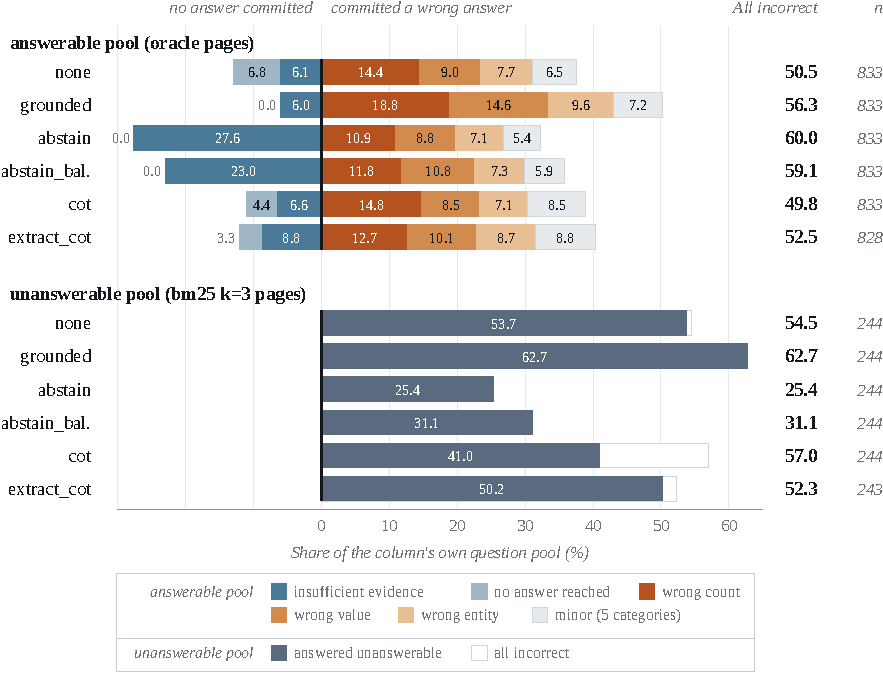
\includegraphics[width=0.72\textwidth]{appendix/figures/error_profile.pdf}
\caption{Error categories by prompt mode on answerable and unanswerable questions.}
\label{fig:app_error_profile}
\end{figure*}

\begin{figure*}[t]
\centering
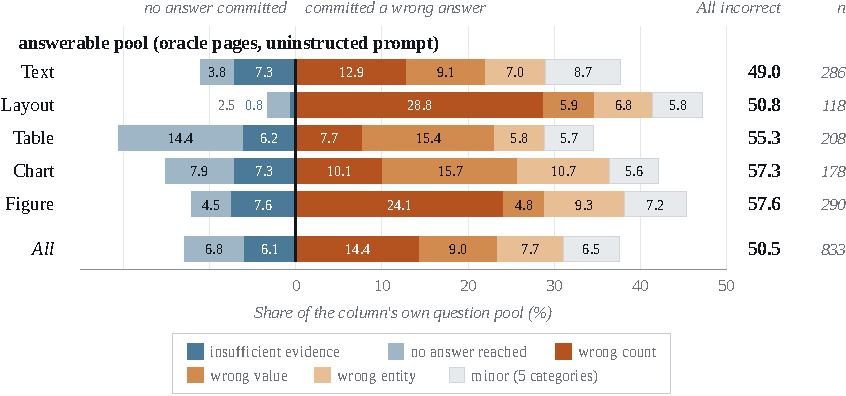
\includegraphics[width=0.69\textwidth]{appendix/figures/error_sources.pdf}
\caption{Error categories by evidence source on answerable questions with no instruction.}
\label{fig:app_error_sources}
\end{figure*}

The taxonomy rubric assigns each incorrect response one error category (Table~\ref{tab:app_error_taxonomy}). Figures~\ref{fig:app_error_profile} and~\ref{fig:app_error_sources} show the share of each category, with responses that commit to no answer on the left and wrong answers on the right.

\paragraph{By Prompt Mode.}
The abstention instructions change the kind of error more than its amount (Figure~\ref{fig:app_error_profile}). Under \texttt{abstain}, refusals on answerable questions rise from 6.1\% to 27.6\% while every wrong-answer category shrinks, and answers to unanswerable questions fall from 53.7\% to 25.4\%. \texttt{grounded} moves in the opposite direction, removing unfinished responses but adding wrong values and counts.

\paragraph{By Evidence Source.}
Wrong counts dominate layout and figure questions, at 28.8\% and 24.1\% (Figure~\ref{fig:app_error_sources}). Table and chart questions fail mainly on values, and table questions most often end without stating an answer.
